\documentclass[11pt]{article}
\usepackage[spanish,es-noshorthands]{babel}
\usepackage[utf8]{inputenc}
\usepackage[T1]{fontenc}
\usepackage{lmodern}
\usepackage{geometry}
\usepackage{graphicx}
\usepackage{amssymb}
\usepackage{xcolor}
\usepackage{listings}
\usepackage{booktabs, tabularx, array}
\usepackage{enumitem}
\usepackage{fancyhdr}
\usepackage{tcolorbox}
\usepackage[hidelinks]{hyperref}
\geometry{letterpaper, margin=2.3cm}
\setlength{\parindent}{0pt}
\setlength{\parskip}{0.55em}
\definecolor{azul}{HTML}{2F4A6D}
\definecolor{fondo}{HTML}{F3F5F8}
\lstset{basicstyle=\ttfamily\small, backgroundcolor=\color{fondo}, frame=single, rulecolor=\color{azul!40},
  columns=fullflexible, keepspaces=true, breaklines=true, showstringspaces=false, extendedchars=true,
  literate={á}{{\'a}}1 {é}{{\'e}}1 {í}{{\'i}}1 {ó}{{\'o}}1 {ú}{{\'u}}1 {ñ}{{\~n}}1 {«}{{\guillemotleft}}1 {»}{{\guillemotright}}1}
\newcommand{\cod}[1]{\texttt{#1}}
\newtcolorbox{nota}{colback=fondo, colframe=azul, boxrule=0.6pt, arc=2pt, left=6pt, right=6pt}
\pagestyle{fancy}\fancyhf{}
\lhead{\small\color{azul} Taller EDEPA 2026 · Generación parametrizada de prácticas}
\rhead{\small\thepage}
\renewcommand{\headrulewidth}{0.4pt}

\begin{document}
\sloppy

\begin{center}
{\LARGE\bfseries\color{azul} Guía del taller}\\[0.4em]
{\large Generación parametrizada de ejercicios de Estadística y Probabilidad\\ con Python, Excel, Jinja2 y \LaTeX}\\[0.5em]
{\normalsize Francisco Antonio Campos Sandí \& Gerardo Córdoba Hernández}\\[0.5em]
{\small IX Encuentro sobre Didáctica de la Estadística, la Probabilidad y el Análisis de Datos (EDEPA 2026)}
\end{center}

\begin{nota}
\textbf{Qué hace este material.} Lee una lista de estudiantes desde Excel y produce, para cada estudiante, una práctica con datos propios y su solución paso a paso. Cada generador entrega dos PDF: las \textbf{prácticas} y las \textbf{soluciones}, que comienzan con una \textbf{hoja de respuestas} para el docente. Todos los nombres de la lista de ejemplo son inventados.
\end{nota}

\begin{center}
\begin{tcolorbox}[colback=white, colframe=azul, boxrule=0.6pt, arc=2pt, width=0.86\linewidth, left=8pt, right=8pt]
\begin{minipage}[c]{3.4cm}
\href{https://github.com/Francisco-Campos-S/Plantilla_Taller_EDEPA_2026}{
\includegraphics[width=3.4cm]{qr_repositorio.png}}
\end{minipage}\hfill
\begin{minipage}[c]{\dimexpr\linewidth-3.9cm}
{\color{azul}\bfseries Repositorio del taller}\par\smallskip
Escanee el código con la cámara del celular para abrir el repositorio, descargar la plantilla y consultar esta guía.\par\smallskip
{\small\url{https://github.com/Francisco-Campos-S/Plantilla_Taller_EDEPA_2026}}
\end{minipage}
\end{tcolorbox}
\end{center}

\tableofcontents

\section{Contenido del repositorio}

\begin{tabularx}{\linewidth}{@{}>{\raggedright\arraybackslash}p{6.3cm}X@{}}
\toprule
\textbf{Archivo} & \textbf{Para qué sirve} \\ \midrule
\cod{generar\_estadistica.py} + \cod{template\_estadistica.tex} & Estadística descriptiva: tres preguntas (estadísticos básicos, moda con valores repetidos y lectura de un gráfico). \\
\cod{generar\_probabilidad.py} + \cod{template\_probabilidad.tex} & Probabilidad: cuatro preguntas (bolsa, dos dados, tabla de $2\times2$ y frecuencia relativa). \\
\cod{generar\_mi\_practica.py} + \cod{template\_mi\_practica.tex} & Plantilla para construir su propio generador (ejemplo: porcentajes). \\
\cod{pruebas.py} & Pruebas automáticas de los cálculos. \\
\cod{lista\_estudiantes\_ficticia.xlsx} & Lista de prueba con 19 nombres inventados. \\
\cod{ejemplos/} & Los cuatro PDF de una corrida con semilla 2026, para comparar. \\
\cod{LEEME\_TALLER.md} & Resumen breve de esta guía. \\ \bottomrule
\end{tabularx}

\begin{figure}[h]
\centering
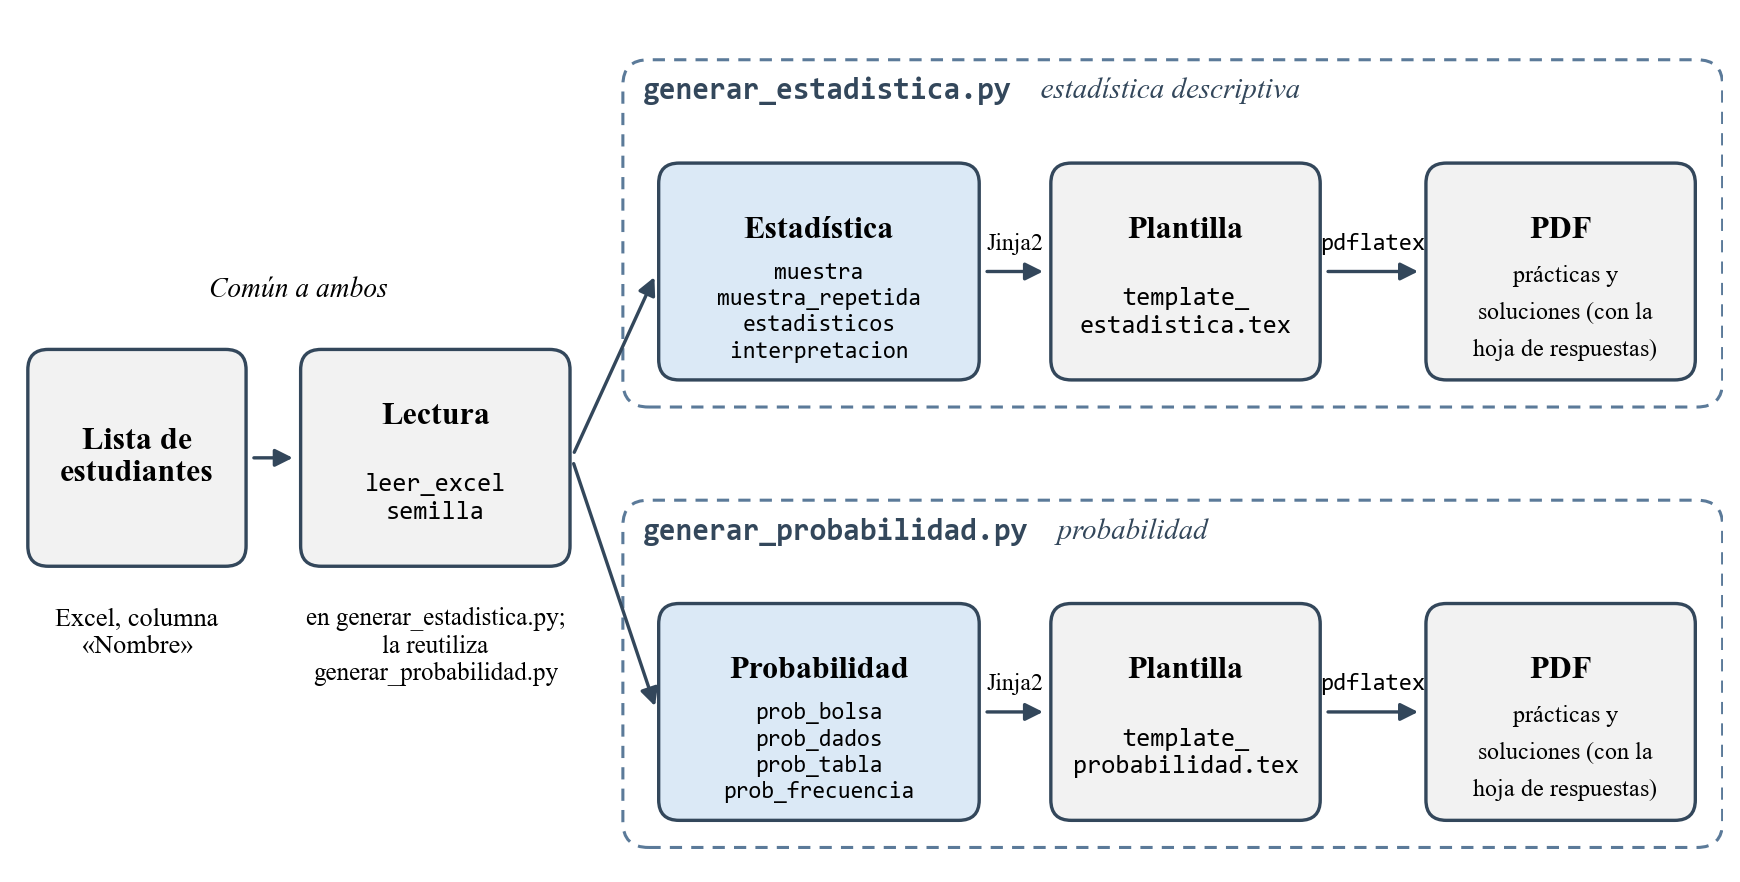
\includegraphics[width=\linewidth]{flujo.png}
\caption{Flujo de los dos generadores: de la lista de estudiantes a los PDF.}
\end{figure}

\section{Instalación (antes del taller)}

\begin{enumerate}[leftmargin=*]
\item \textbf{Python 3} (3.10 o posterior): \url{https://www.python.org/downloads/}. En Windows, marque la casilla \emph{Add Python to PATH} durante la instalación.
\item \textbf{\LaTeX} con el paquete \cod{pgfplots}: MiKTeX (\url{https://miktex.org/}) en Windows o TeX Live en Linux y macOS. En MiKTeX, active la instalación automática de paquetes faltantes.
\item \textbf{Librerías de Python}. En una terminal (en Windows, PowerShell), ejecute:
\begin{lstlisting}
pip install pandas openpyxl jinja2
\end{lstlisting}
\item \textbf{Descargue el material}: en GitHub, botón \emph{Code} $\rightarrow$ \emph{Download ZIP}, y descomprima la carpeta; o bien
\begin{lstlisting}
git clone https://github.com/Francisco-Campos-S/Plantilla_Taller_EDEPA_2026.git
\end{lstlisting}
Repositorio: \url{https://github.com/Francisco-Campos-S/Plantilla_Taller_EDEPA_2026}
\item \textbf{Compruebe la instalación} desde la carpeta descargada:
\begin{lstlisting}
python pruebas.py
\end{lstlisting}
Debe terminar con \cod{OK}. Si aparece un error, revise la sección~\ref{sec:problemas}.
\end{enumerate}

\section{Primera corrida}

\begin{enumerate}[leftmargin=*]
\item Abra una terminal en la carpeta del material y ejecute \cod{python generar\_estadistica.py}.
\item En la ventana, pulse \emph{Seleccionar archivo} y elija \cod{lista\_estudiantes\_ficticia.xlsx}. El programa busca la fila cuyo encabezado es \textbf{Nombre}, aunque no esté en la primera fila, y genera una práctica por cada nombre.
\item La ventana muestra el avance. Al terminar, la carpeta \cod{practicas\_estadistica/} contiene \cod{practicas\_estadistica.pdf} y \cod{soluciones\_estadistica.pdf}.
\item Repita con \cod{python generar\_probabilidad.py}; los PDF aparecen en \cod{practicas\_probabilidad/}.
\item Compare la práctica de un estudiante con su solución y con su fila en la hoja de respuestas.
\end{enumerate}

\begin{figure}[h]
\centering
\begin{minipage}{0.48\linewidth}\centering
\fbox{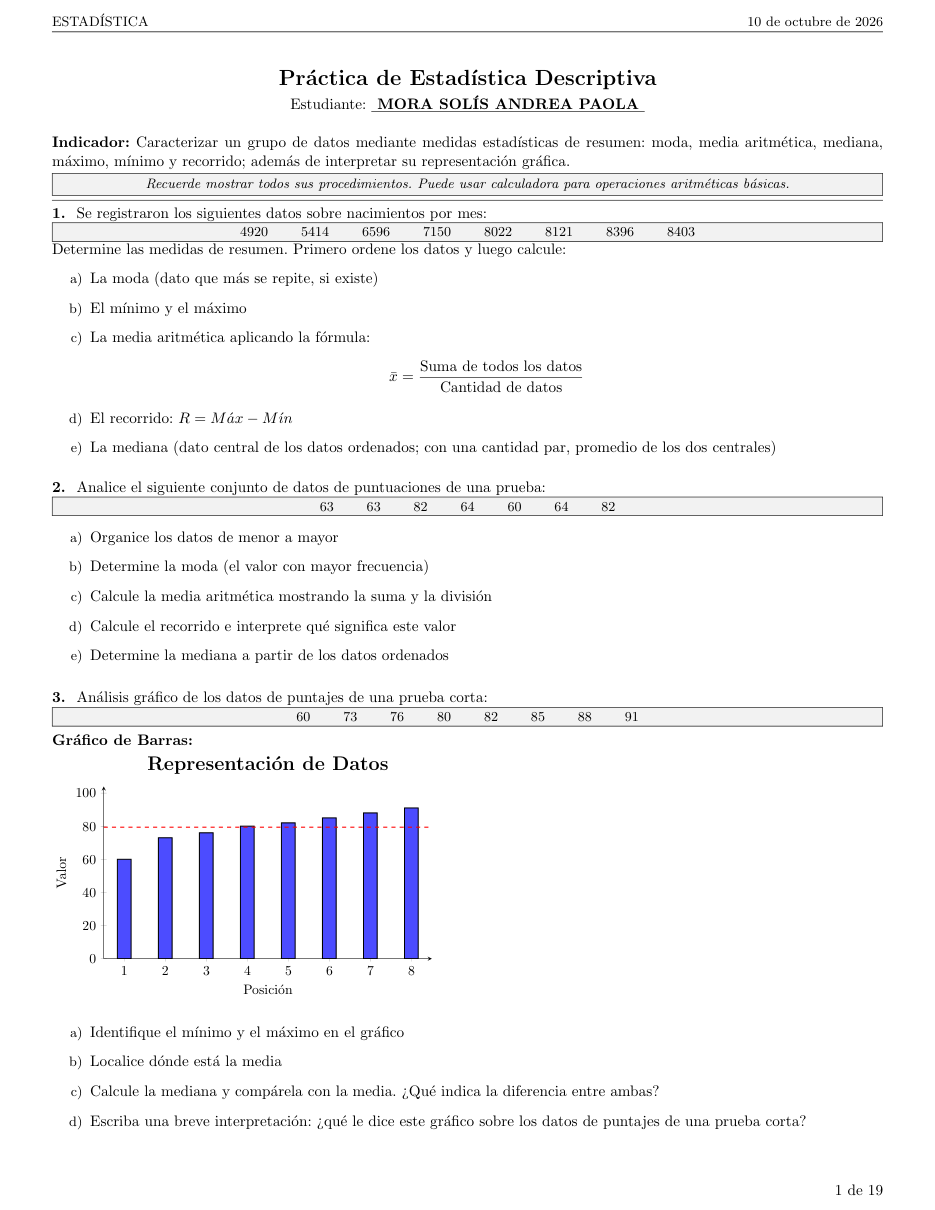
\includegraphics[width=0.95\linewidth]{ej_practica.png}}\\[0.2em]{\small (a) Práctica de un estudiante}
\end{minipage}\hfill
\begin{minipage}{0.48\linewidth}\centering
\fbox{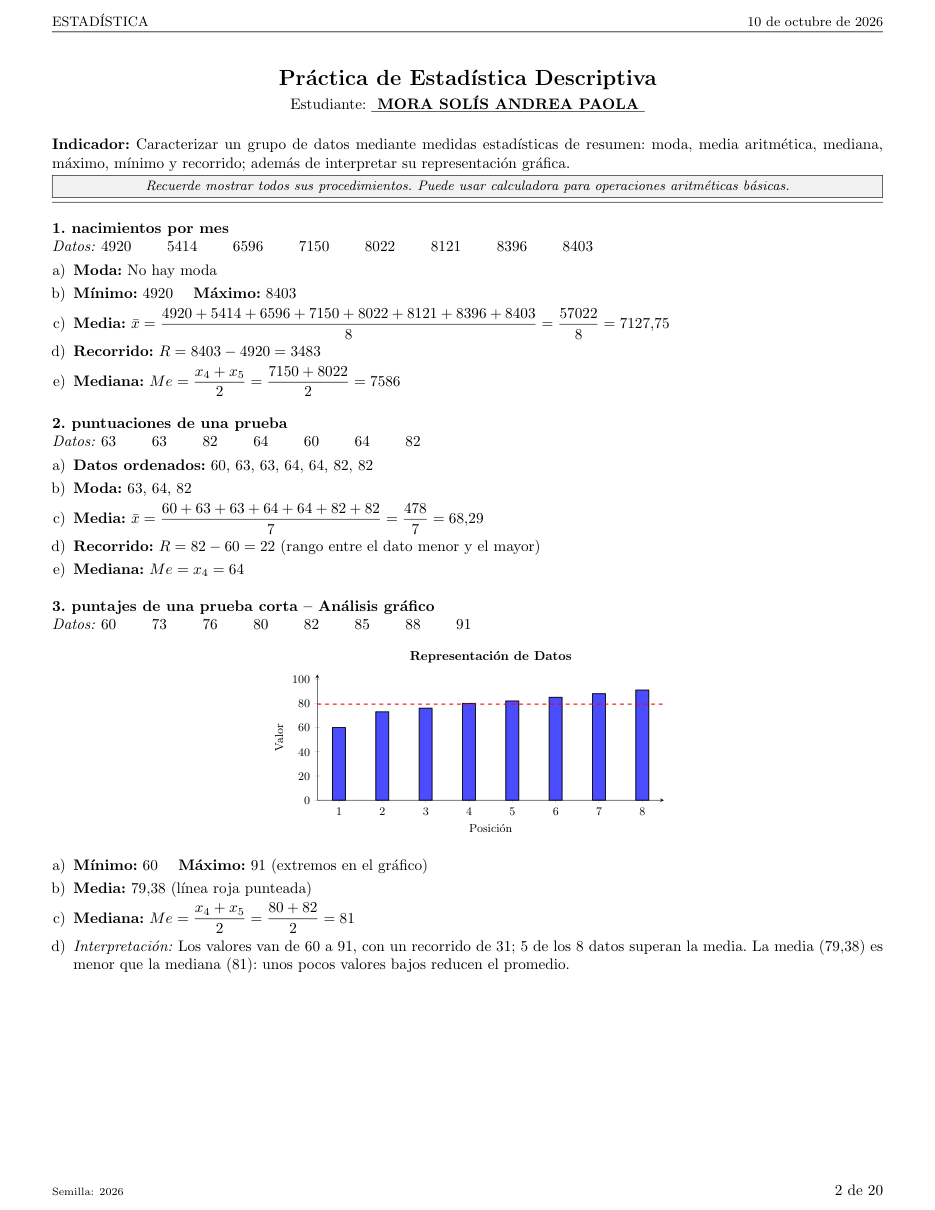
\includegraphics[width=0.95\linewidth]{ej_solucion.png}}\\[0.2em]{\small (b) Su solución, con los mismos datos}
\end{minipage}
\caption{Primera página de las prácticas y de las soluciones (corrida con semilla 2026).}
\end{figure}

\begin{figure}[h]
\centering
\fbox{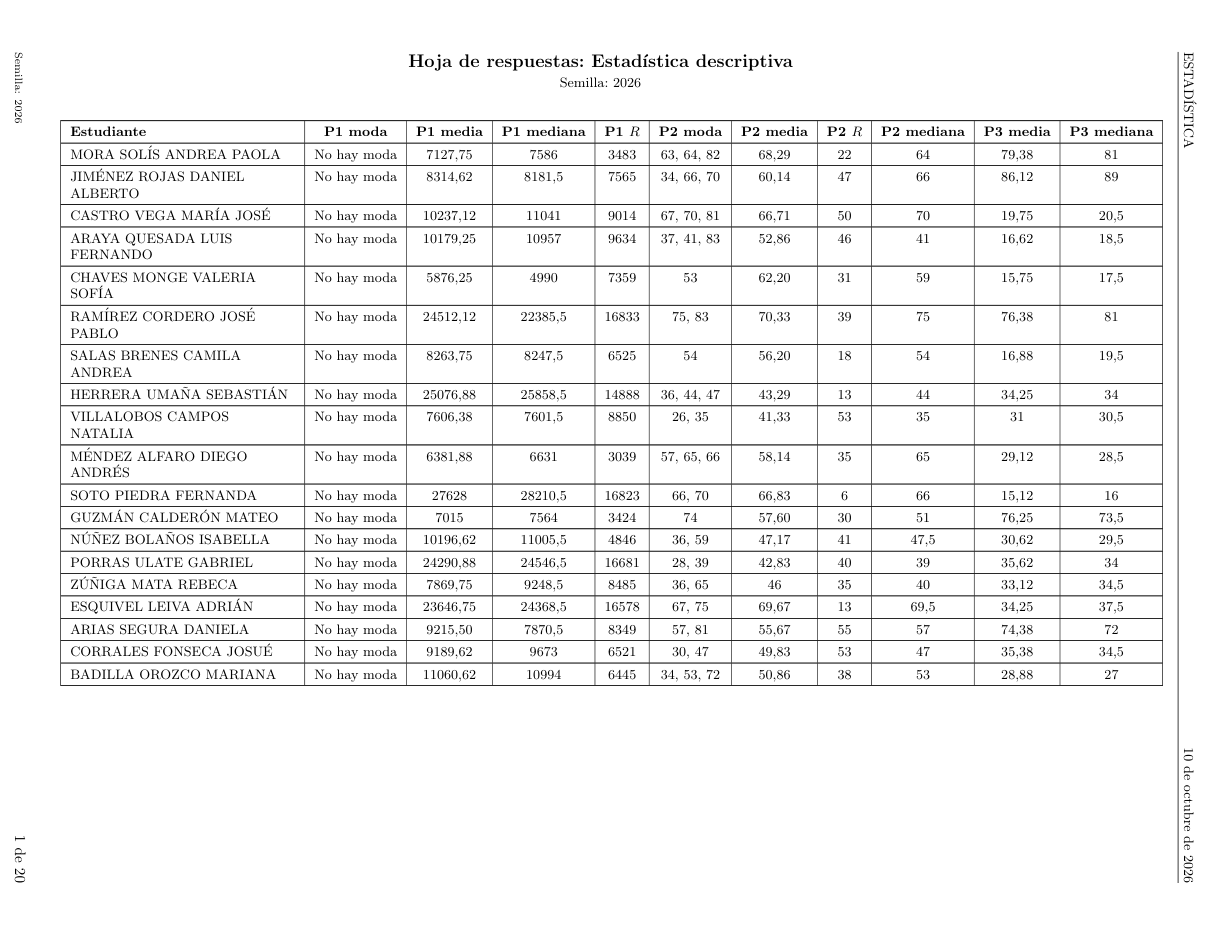
\includegraphics[width=0.85\linewidth]{ej_hoja.png}}
\caption{Hoja de respuestas al inicio del PDF de soluciones: una fila por estudiante.}
\end{figure}

\begin{nota}
\textbf{La semilla.} Cada corrida usa una semilla aleatoria que queda impresa al pie de las soluciones y en la hoja de respuestas. Con la misma lista, la misma plantilla y la misma semilla se obtienen exactamente los mismos números; así se puede reconstruir la práctica de cualquier estudiante.
\end{nota}

\section{Cómo funciona el código}

\subsection{Funciones comunes (en \cod{generar\_estadistica.py})}
\begin{itemize}[leftmargin=*]
\item \cod{leer\_excel(path)}: recorre las filas hasta encontrar «Nombre», toma esa fila como encabezado y devuelve los registros siguientes; las celdas vacías se omiten.
\item \cod{esc(texto)}: traduce los caracteres que \LaTeX{} interpreta como órdenes (\verb|\|, \verb|&|, \verb|%|, \verb|$|, \verb|#|, \verb|_|, \verb|{|, \verb|}|, \verb|~|, \verb|^|, \verb|<|, \verb|>|) para que un nombre como \cod{Ana\_Perez \& 100\%} no rompa la compilación.
\item \cod{procesar(...)}: fija la semilla, llama a la función de datos de cada estudiante, rellena la plantilla con Jinja2 y compila con \cod{pdflatex}. La reutilizan los otros dos generadores.
\end{itemize}

\subsection{Estadística descriptiva}
\begin{itemize}[leftmargin=*]
\item \cod{muestra(n, lo, hi)}: $n$ enteros aleatorios ordenados entre \cod{lo} y \cod{hi}. Las preguntas 1 y 3 usan $n=8$.
\item \cod{muestra\_repetida()}: de 5 a 7 datos con al menos un valor repetido; la pregunta 2 siempre tiene moda.
\item \cod{estadisticos(datos)}: suma, media, mediana, mínimo, máximo, recorrido y moda. Si ningún valor se repite, o si todos se repiten el mismo número de veces (1, 1, 2, 2, 5, 5), la salida es «No hay moda».
\item \cod{interpretacion(...)}: redacta la lectura del gráfico comparando la media y la mediana.
\end{itemize}

\subsection{Probabilidad}
\begin{itemize}[leftmargin=*]
\item \cod{prob\_bolsa}: regla de Laplace, complemento y dos extracciones sin reposición.
\item \cod{prob\_dados}: cuenta los casos favorables entre los 36 pares ordenados.
\item \cod{prob\_tabla}: tabla de $2\times2$ con probabilidad marginal, conjunta y condicional, y discusión de la independencia.
\item \cod{prob\_frecuencia}: frecuencia relativa de una cara en lanzamientos simulados, comparada con $1/6$.
\end{itemize}
Las probabilidades se calculan con fracciones exactas (\cod{Fraction}) y se muestran simplificadas y en decimal.

\section{Construir su propio generador}

Abra \cod{generar\_mi\_practica.py}. Tiene tres partes marcadas con \cod{EDITAR}:

\textbf{1. Contextos.} Situaciones cerradas con sus rangos de valores:
\begin{lstlisting}[language=Python]
CONTEXTOS = [
    ("estudiantes de un colegio", "viajan en autobús", 40, 120),
    ("visitantes de un parque nacional", "son extranjeros", 50, 200),
]
\end{lstlisting}

\textbf{2. Datos y solución de cada estudiante.} La función devuelve un diccionario; cada clave es una variable de la plantilla. Pase por \cod{ge.esc()} todo texto que vaya a \LaTeX:
\begin{lstlisting}[language=Python]
def datos_estudiante(idx, nombre):
    poblacion, rasgo, lo, hi = random.choice(CONTEXTOS)
    total = random.randint(lo, hi)
    k = random.randint(1, total - 1)
    p = k * 100 / total
    return {"estudiante": ge.esc(nombre), "total": total, "k": k,
            "porcentaje": ge.num(p), ...}
\end{lstlisting}

\textbf{3. Hoja de respuestas.} Columnas que aparecerán al inicio de las soluciones:
\begin{lstlisting}[language=Python]
CLAVE = [("Encuestados", lambda d: str(d["total"])),
         ("Porcentaje",  lambda d: d["porcentaje"] + r"\,\%")]
\end{lstlisting}

\textbf{4. La plantilla.} En \cod{template\_mi\_practica.tex}, el enunciado va en el bloque \verb|{% if modo == 'practicas' %}| y la solución en el bloque \verb|{% else %}|. Las variables se escriben entre llaves dobles:
\begin{lstlisting}
\textbf{1. } En una encuesta a {{ total }} {{ poblacion }}, {{ k }} {{ rasgo }}.
\end{lstlisting}

Ejecute \cod{python generar\_mi\_practica.py}; los PDF aparecen en \cod{practicas\_mi\_practica/}.

\begin{nota}
\textbf{Consejos.} Cambie una sola cosa a la vez y vuelva a ejecutar. Revise al menos tres estudiantes comparando la práctica con la solución. Conserve la semilla de la corrida que entregue.
\end{nota}

\section{Problemas frecuentes}\label{sec:problemas}

\begin{tabularx}{\linewidth}{@{}>{\raggedright\arraybackslash}p{5.2cm}X@{}}
\toprule
\textbf{Síntoma} & \textbf{Qué hacer} \\ \midrule
\cod{ModuleNotFoundError: pandas} (o \cod{jinja2}, \cod{openpyxl}) & Ejecute \cod{pip install pandas openpyxl jinja2}. \\
\cod{pdflatex} no se reconoce & Instale MiKTeX o TeX Live y abra una terminal nueva. \\
El PDF no aparece & Abra el archivo \cod{.log} de la carpeta de salida y busque la primera línea que empieza con \cod{!}. \\
MiKTeX pide instalar un paquete & Acepte; la primera compilación descarga \cod{pgfplots} y otros paquetes. \\
La ventana dice \cod{Error: Sin columna 'Nombre'} & La lista debe tener una celda con el texto exacto \cod{Nombre} sobre la columna de nombres. \\
Un nombre con símbolos rompe el PDF & Compruebe que el texto pasa por \cod{ge.esc()} en \cod{datos\_estudiante}. \\ \bottomrule
\end{tabularx}

\section{Lista de cotejo para revisar un ajuste}

\begin{tabularx}{\linewidth}{@{}Xccc@{}}
\toprule
\textbf{Criterio} & \textbf{Sí} & \textbf{No} & \textbf{Observaciones} \\ \midrule
El objetivo de aprendizaje de la pregunta sigue siendo el mismo. & $\square$ & $\square$ & \\
El contexto es pertinente para el grupo y sus unidades son claras. & $\square$ & $\square$ & \\
Los rangos producen datos verosímiles para el contexto. & $\square$ & $\square$ & \\
La consigna nombra la medida o la probabilidad que se pide. & $\square$ & $\square$ & \\
La solución coincide con el enunciado en al menos tres estudiantes revisados. & $\square$ & $\square$ & \\
La moda, la mediana y el redondeo siguen la convención declarada. & $\square$ & $\square$ & \\
Las probabilidades aparecen como fracción simplificada y decimal. & $\square$ & $\square$ & \\
La corrida registra la semilla y \cod{python pruebas.py} termina sin fallos. & $\square$ & $\square$ & \\ \bottomrule
\end{tabularx}

\section{Privacidad y uso responsable}

\begin{itemize}[leftmargin=*]
\item Use la lista real de su grupo solo en su computadora; no la suba a este repositorio ni la envíe a servicios externos.
\item El generador no transmite datos: todo el cálculo y la compilación ocurren en su equipo.
\item Si usa inteligencia artificial para redactar contextos o consignas, revise el resultado, declare su uso y conserve la responsabilidad del material.
\end{itemize}

\end{document}
